\chapter{Analisi del sistema}

\section{Introduzione}
In questo documento effetturemo l'analisi del sistema, ci avvarremo del linguaggio \gls{uml} per formalizzare i requisiti descritti nel documento \docref{cha:specifica_requisiti} e in parte espressi nei casi d'uso nella \docref{cha:usecase}.
Effettueremo la formalizzazione esclusivamente delle parti prinicpali del sistema, in particolare andremo a realizzare i seguenti diagrammi:
\begin{itemize}
	\item Diagrammi di attività
	\item Diagramma dei package
	\item Diagrammi delle classi
	\item Diagrammi di sequenza
\end{itemize}

\section{Diagrammi di attività}
I diagrammi di attività descrivono il comportamento nel tempo di un particolare elemento. Con essi si modella l’interazione e la fusione dei flussi principali con i flussi alternativi dei casi d’uso. Questo viene fatto per rendere più visibili le varie ramificazioni che i flussi possono avere all’interno di un caso d’uso. Non verranno rappresentati tutti i diagrammi di attività, ma solo quelli corrispondenti ai casi d'uso principali.
\begin{center}
	\begin{tabularx}{\textwidth}{ l X } 
		\toprule
		\formattaTitoloTab{ID} & \formattaTitoloTab{Caso d'uso di riferimento} \\
		\cmidrule(l{\cmidrulekern}r{\cmidrulekern}){1-2}
		\newAttivita{da:login}{\formattaAT}{Login} & \getIDTitletodesc{cu:login} \\ 
		\addlinespace[1em] 
		\newAttivita{da:logout}{\formattaAT}{Logout} & \getIDTitletodesc{cu:logout} \\ 
		\addlinespace[1em] 
		\newAttivita{da:iscrizione}{\formattaAT}{Iscrizione} & \getIDTitletodesc{cu:iscrizionePortale} \\
		 													 & \getIDTitletodesc{cu:iscrizioneSocial} \\
															 & \getIDTitletodesc{cu:iscrizioneApprovazione} \\ 
		\addlinespace[1em] 
		\newAttivita{da:approvazione}{\formattaAT}{Approvazione iscrizione} & \getIDTitletodesc{cu:approvazioneIscrizione} \\ 
		\addlinespace[1em]
		\newAttivita{da:schedaprodotto}{\formattaAT}{Inserimento scheda prodotto} & \getIDTitletodesc{cu:personalizzaVetrinaInsProd} \\
		\addlinespace[1em]
		\newAttivita{da:ricerche}{\formattaAT}{Ricerche} & \getIDTitletodesc{cu:ricercaProdotto} \\
														 & \getIDTitletodesc{cu:ricercaNotizia} \\
														 & \getIDTitletodesc{cu:ricercaProfilo} \\
		\addlinespace[1em]
		\newAttivita{da:valrec}{\formattaAT}{Inserimento valutazione e recensione} & \getIDTitletodesc{cu:inserisciValutazioneProdotto} \\
																				   & \getIDTitletodesc{cu:inserisciRecensioneProdotto}\\
		\addlinespace[1em]
		\newAttivita{da:oprec}{\formattaAT}{Operazioni recensione} & \getIDTitletodesc{cu:modificaRecensioneProdotto}\\
																   & \getIDTitletodesc{cu:eliminaRecensioneProdotto}\\
																   & \getIDTitletodesc{cu:commentoRecensione}\\
																   & \getIDTitletodesc{cu:giudizioRecensione}\\ 
																   & \getIDTitletodesc{cu:modificaGiudizioRecensione}\\ 
		\bottomrule
	\end{tabularx}
\end{center}

\linkedSubsection{da:login}
\begin{center}
			\includegraphics[width=\textwidth]{assets/visualParadigm/attivita/login}
\end{center}

\linkedSubsection{da:logout}
\begin{center}
	\includegraphics[width=\textwidth]{assets/visualParadigm/attivita/logout}
\end{center}

\linkedSubsection{da:iscrizione}
\begin{center}
	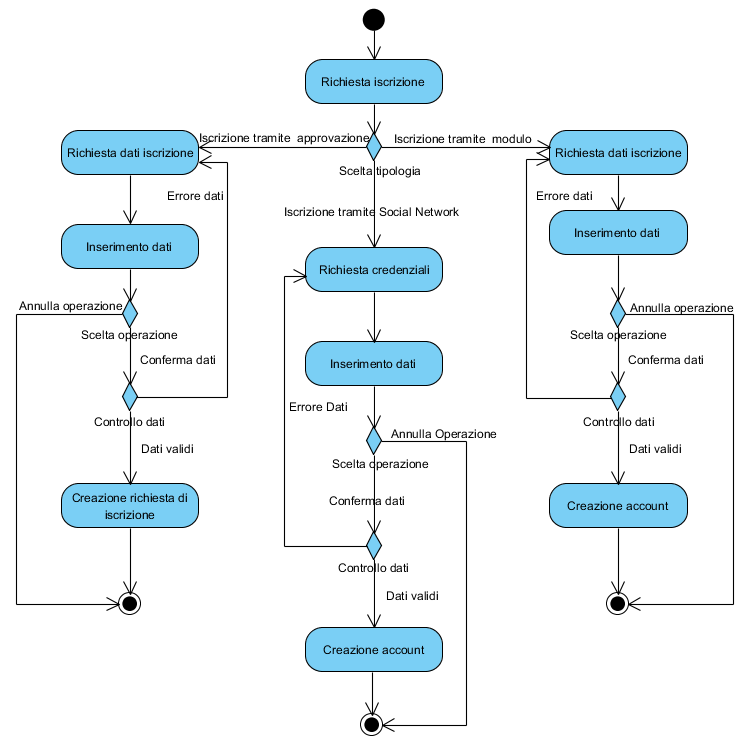
\includegraphics[width=\textwidth]{assets/visualParadigm/attivita/iscrizioni}
\end{center}

\linkedSubsection{da:approvazione}
\begin{center}
	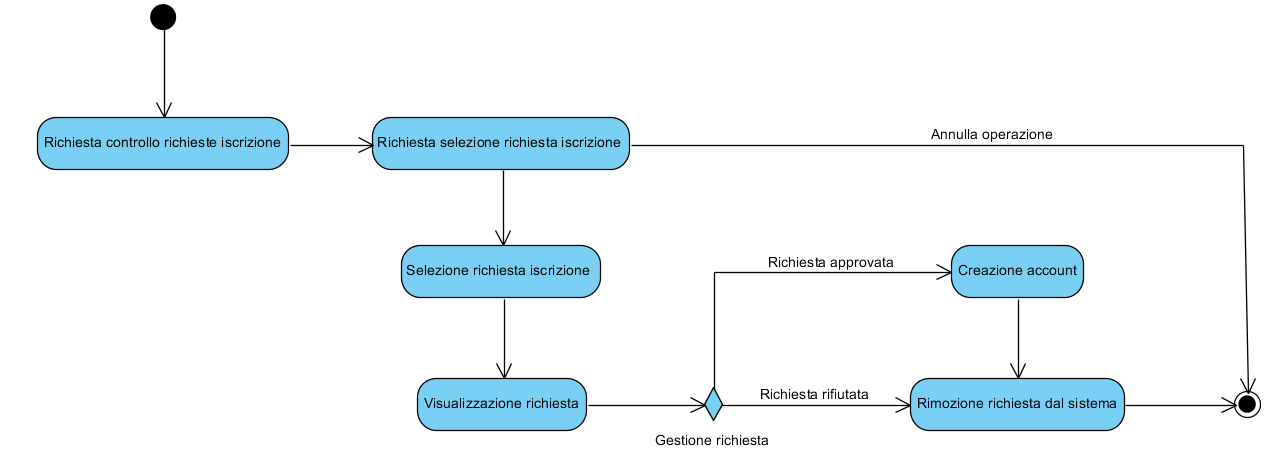
\includegraphics[width=\textwidth]{assets/visualParadigm/attivita/approvazioneIscrizione}
\end{center}

\linkedSubsection{da:schedaprodotto}
\begin{center}
	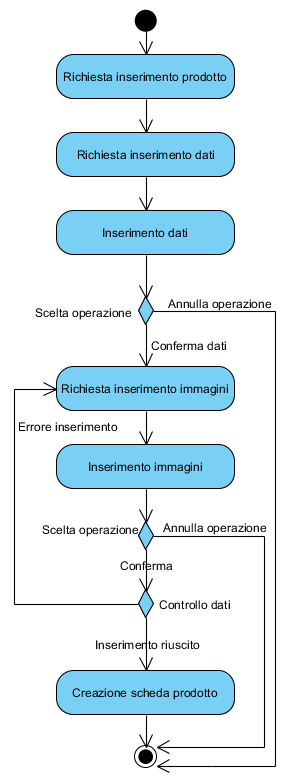
\includegraphics[width=0.5\textwidth]{assets/visualParadigm/attivita/schedaprodotto}
\end{center}

\linkedSubsection{da:ricerche}
\begin{center}
	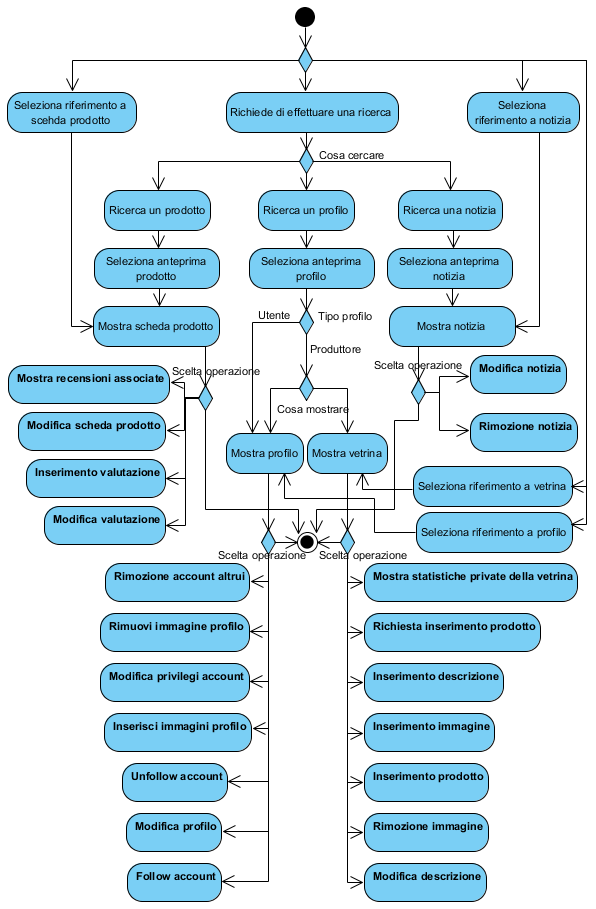
\includegraphics[width=0.95\textwidth]{assets/visualParadigm/attivita/ricerche}
\end{center}

\linkedSubsection{da:valrec}
\begin{center}
	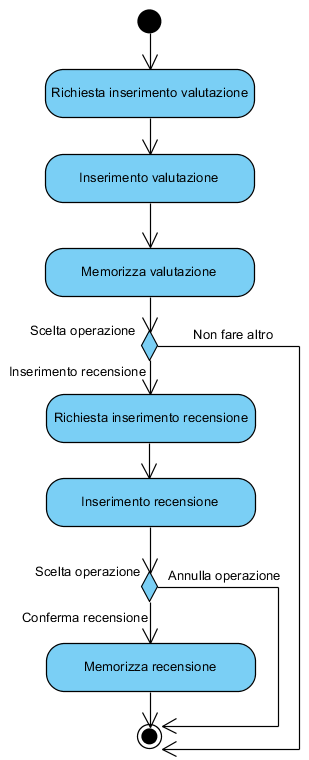
\includegraphics[width=0.5\textwidth]{assets/visualParadigm/attivita/valutazioneRecensione}
\end{center}

\linkedSubsection{da:oprec}
\begin{center}
	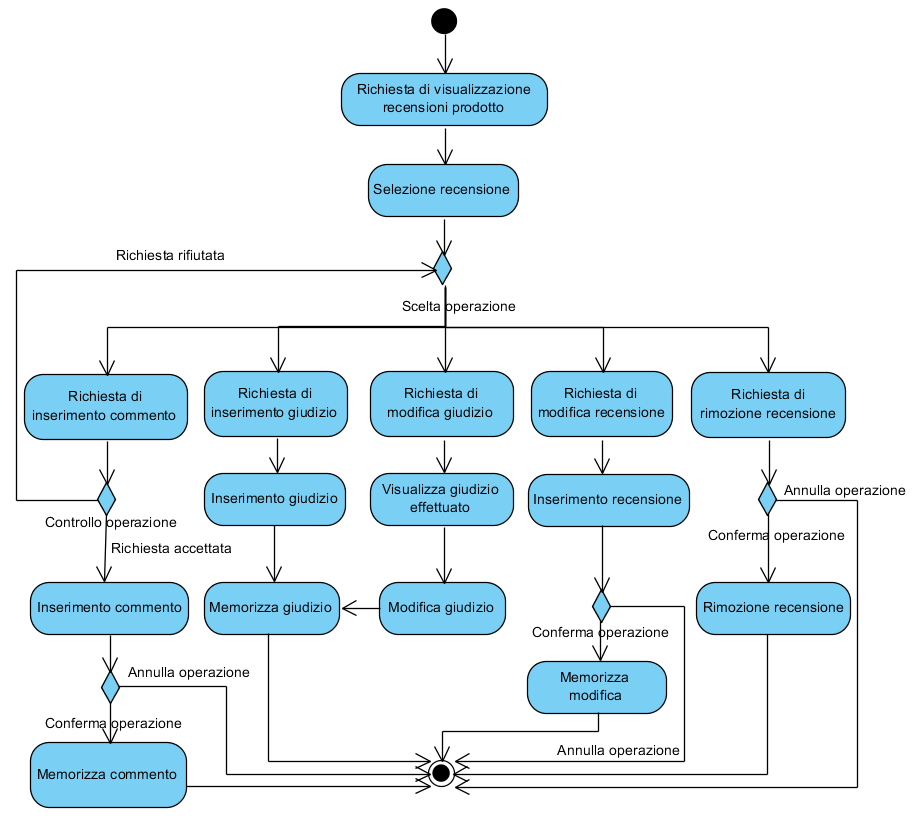
\includegraphics[width=\textwidth]{assets/visualParadigm/attivita/mostraRecensioni}
\end{center}

\begin{landscape}
\section{Diagramma dei package}
Il diagramma dei package sono diagrammi di struttura che descrive i package del sistema e le relazioni tra essi.
Un Package è uno spazio dei nomi utilizzato per raggruppare elementi che sono in relazione semantica tra loro.
\begin{center}
			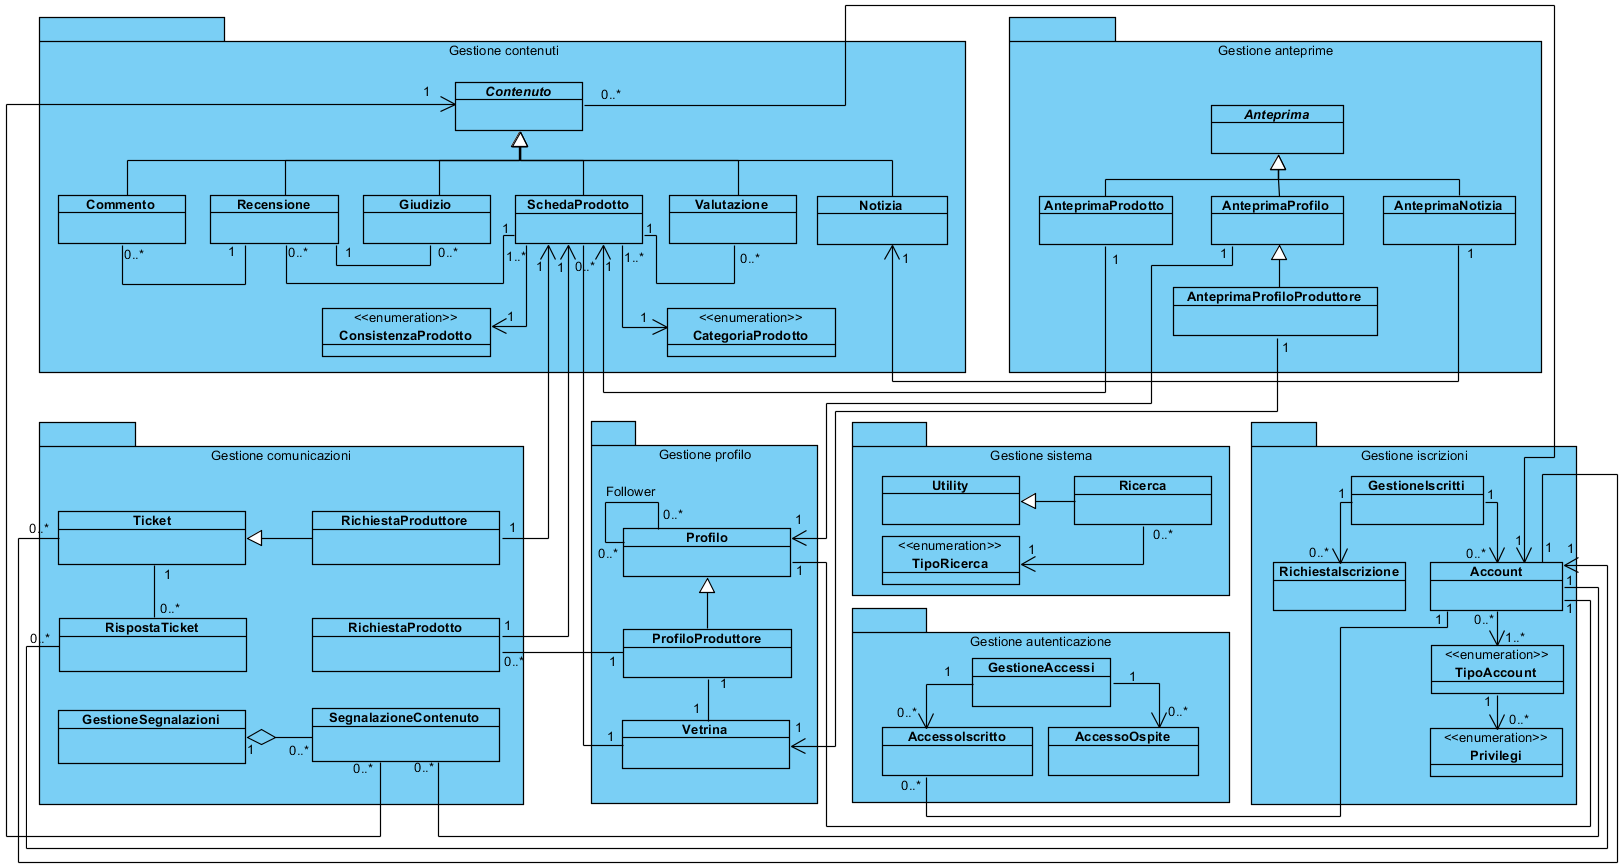
\includegraphics[width=\linewidth]{assets/visualParadigm/package/DiagrammaPacakage}
\end{center}
\end{landscape}

\section{Diagrammi delle classi}
I diagrammi delle classi servono a modellare la relazione tra le entità del sistema, rappresentate come classi.
Una classe è composta da delle caratteristiche che la descrivono (attributi) e delle elaborazioni che vengono eseguite (metodi). 
Le classi servono ad identificare chi fa che cosa e come all’interno del sistema. Queste possono avere relazioni tra loro, le quali sono rappresentate con le associazioni. La cardinalità di un’associazione esprime il numero di oggetti di una certa classe che prendono parte all’associazione.
È inoltre possibile associare una nota ad una classe per descrivere il modello che la classe definisce.
Di seguito sono elencati i diagrammi di sequenza, non verranno riportati tutti i diagrammi di sequenza, ma solo quelli corrispondenti ai casi d'uso principali.
\begin{itemize}
	\item \newPKG{pkg:GestioneAnteprime}{\formattaPKG}{Gestione anteprima}
	\item \newPKG{pkg:GestioneAutenticazione}{\formattaPKG}{Gestione autenticazione}
	\item \newPKG{pkg:GestioneIscritti}{\formattaPKG}{Gestione iscritti}
	\item \newPKG{pkg:GestioneTicket}{\formattaPKG}{Gestione ticket}
	\item \newPKG{pkg:GestioneProfilo}{\formattaPKG}{Gestione profilo}
	\item \newPKG{pkg:GestioneContenuti}{\formattaPKG}{Gestione contenuti}
	\item \newPKG{pkg:GestioneSistema}{\formattaPKG}{Gestione sistema}
\end{itemize}

\linkedSubsection{pkg:GestioneAnteprime}
\begin{center}
			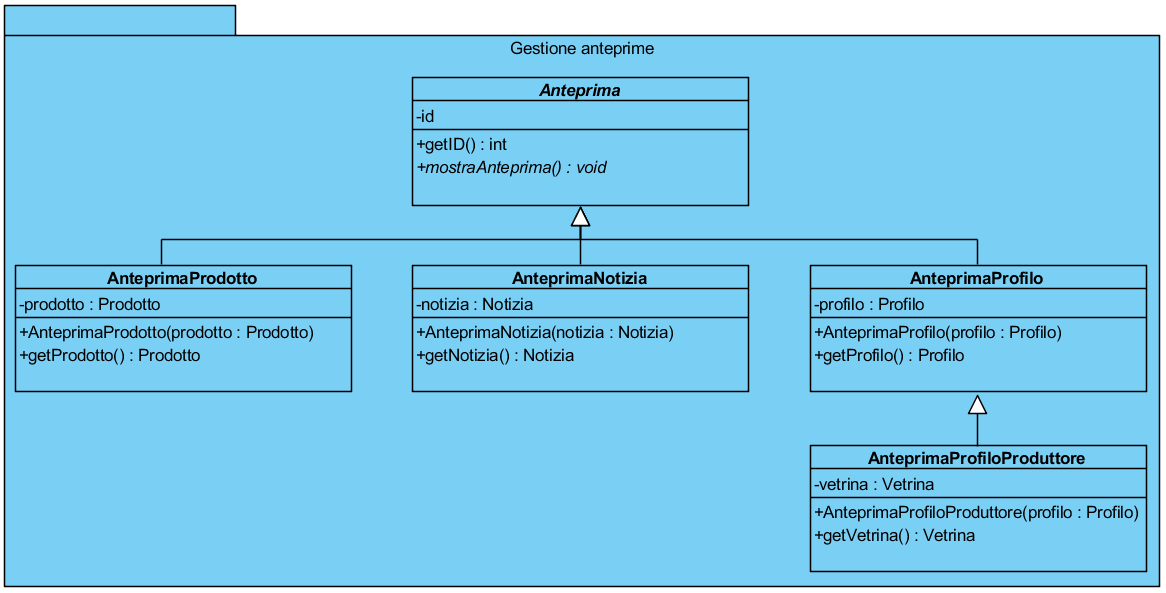
\includegraphics[width=\textwidth]{assets/visualParadigm/classi/GestioneAnteprime}
\end{center}

\linkedSubsection{pkg:GestioneAutenticazione}
\begin{center}
			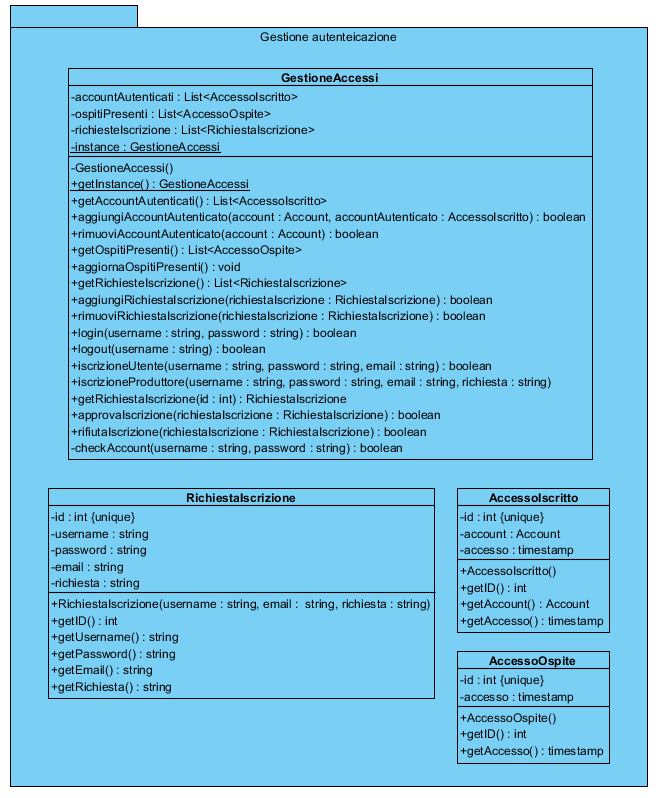
\includegraphics[width=\textwidth]{assets/visualParadigm/classi/GestioneAutenticazione}
\end{center}

\linkedSubsection{pkg:GestioneIscritti}
\begin{center}
			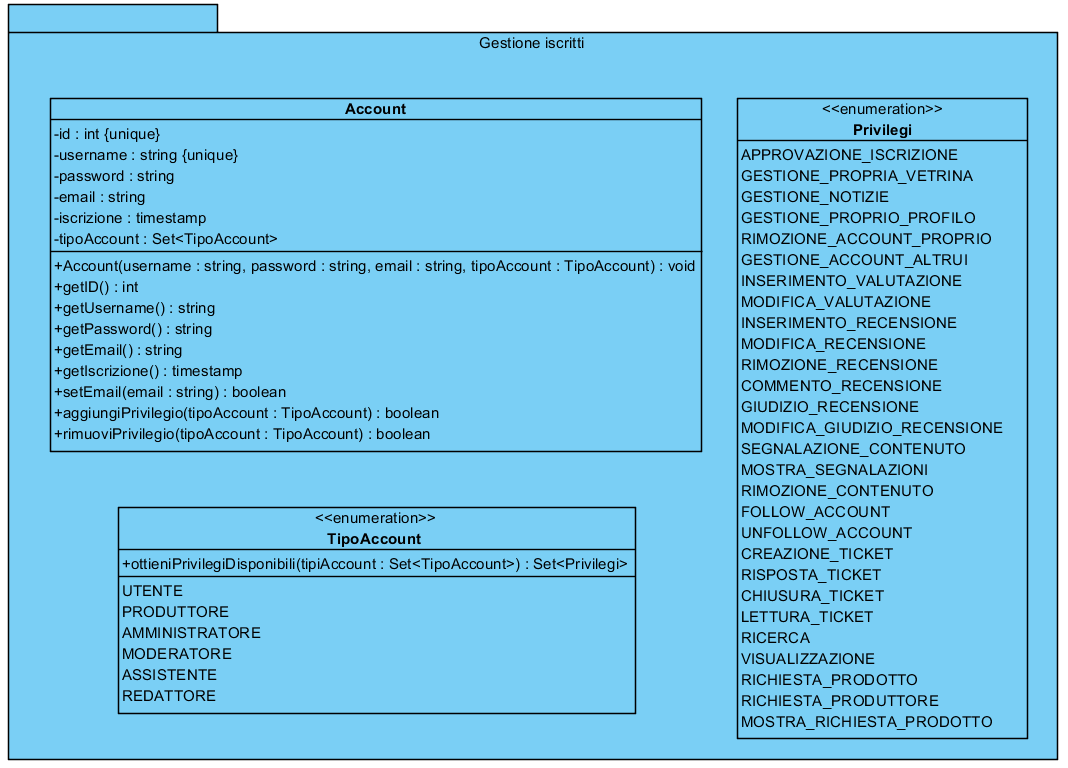
\includegraphics[width=\textwidth]{assets/visualParadigm/classi/GestioneIscritti}
\end{center}

\linkedSubsection{pkg:GestioneTicket}
\begin{center}
			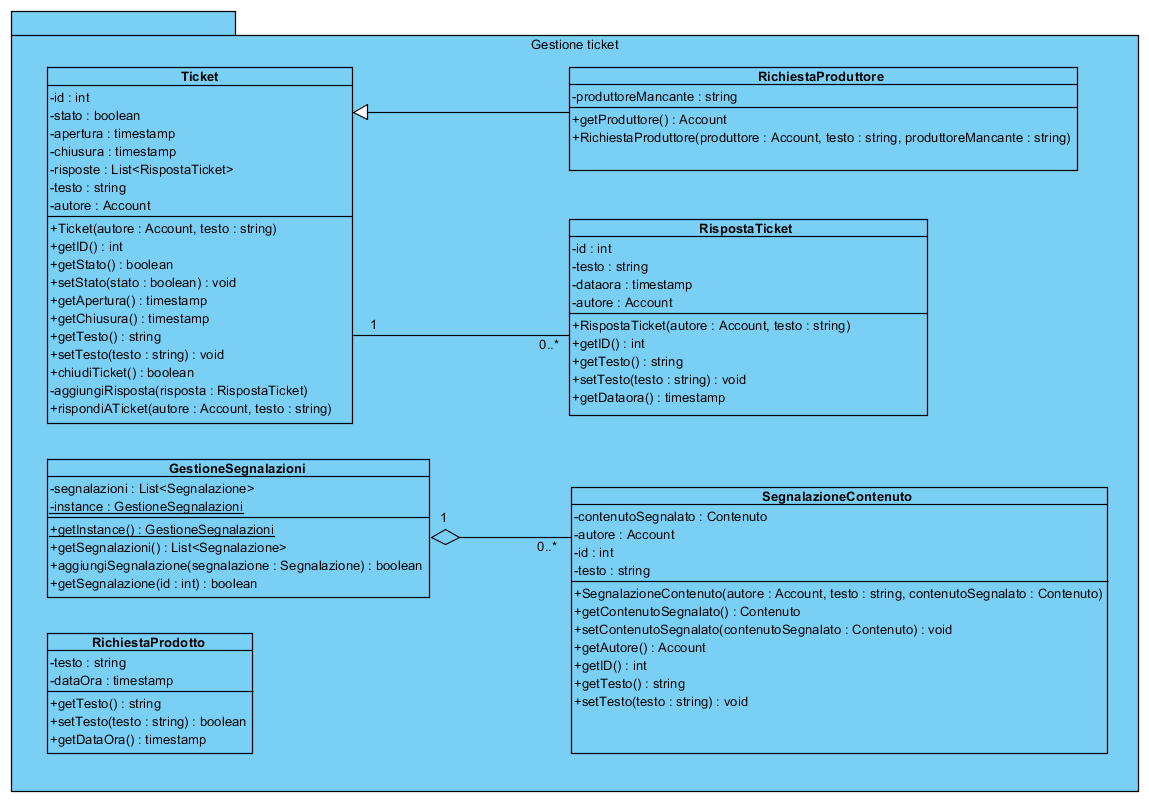
\includegraphics[width=\textwidth]{assets/visualParadigm/classi/GestioneTicket}
\end{center}

\begin{landscape}
\linkedSubsection{pkg:GestioneProfilo}
\begin{center}
			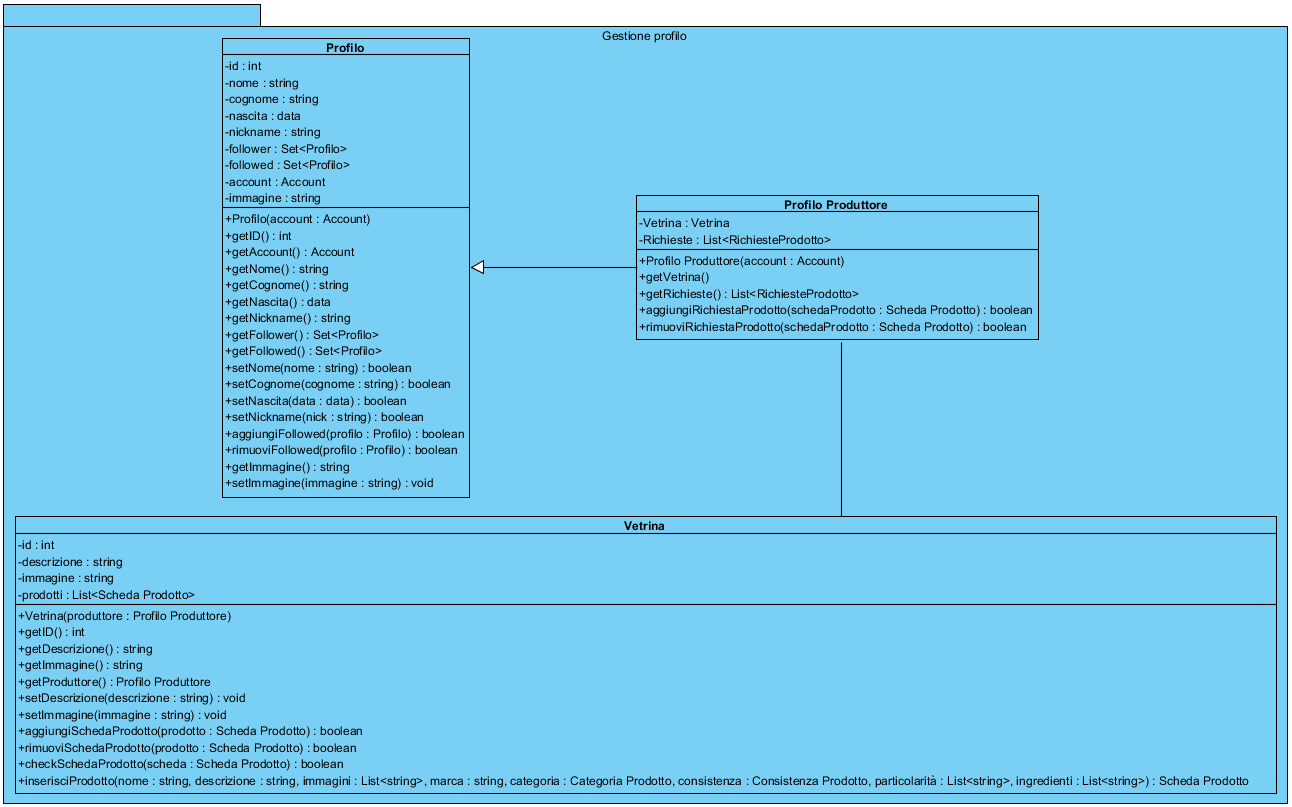
\includegraphics[width=1.1\linewidth]{assets/visualParadigm/classi/GestioneProfilo}
\end{center}
\end{landscape}

\begin{landscape}
\linkedSubsection{pkg:GestioneContenuti}
\begin{center}
			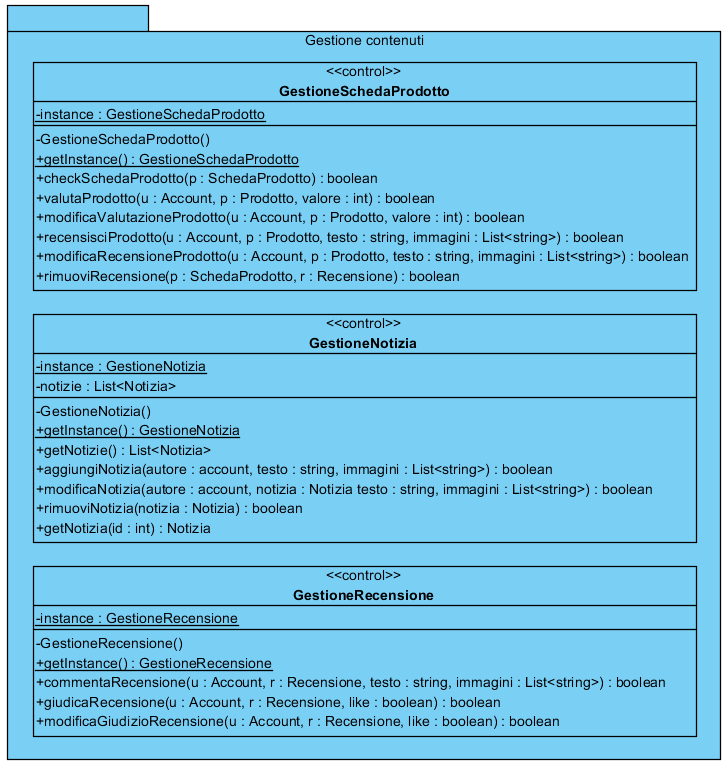
\includegraphics[width=1.1\linewidth]{assets/visualParadigm/classi/GestioneContenuti}
\end{center}
\end{landscape}

\linkedSubsection{pkg:GestioneSistema}
\begin{center}
			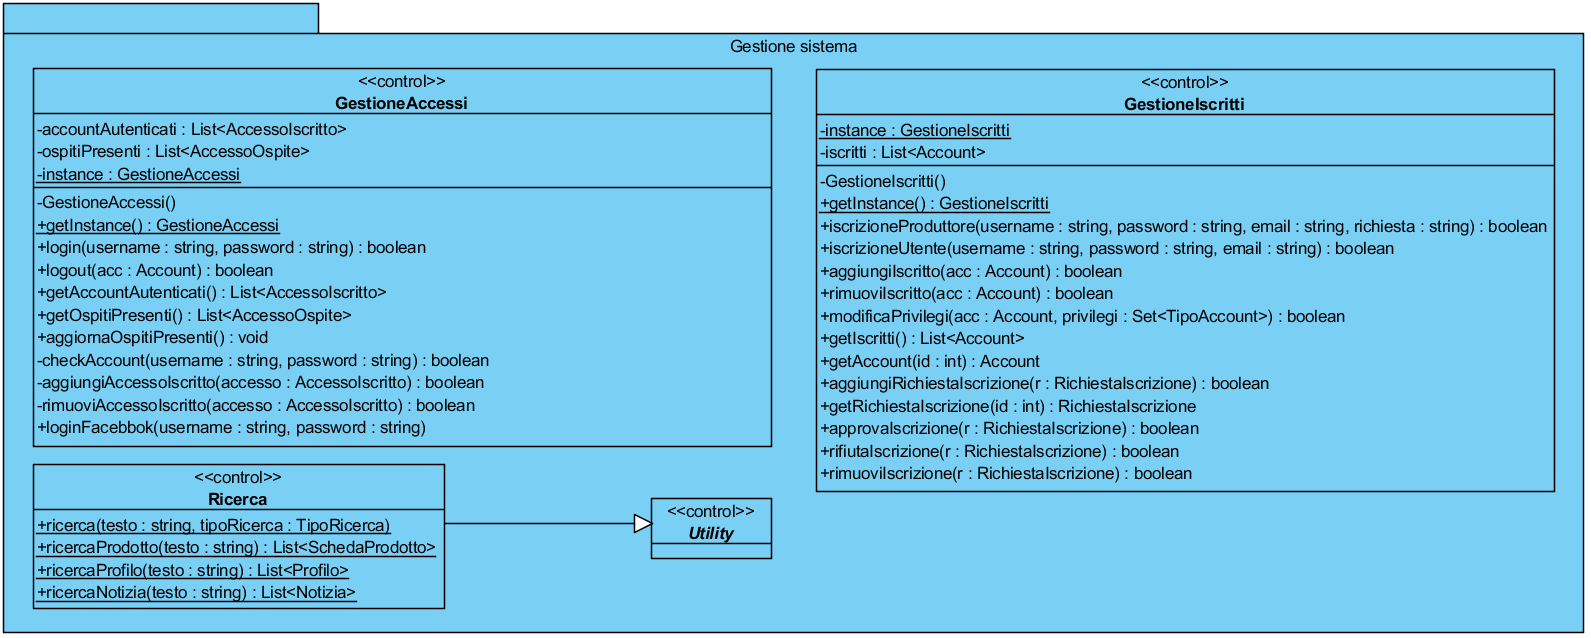
\includegraphics[width=\textwidth]{assets/visualParadigm/classi/GestioneSistema}
\end{center}


\section{Diagrammi di sequenza}
I diagrammi di sequenza descrivono le interazioni tra gli oggetti organizzate in sequenza temporale. Ogni caso d’uso contiene al suo interno diversi diagrammi di sequenza. Rappresenteremo solo le sequenze principali.
Un diagramma di sequenza è costituito da:
\begin{itemize}
	\item Gli oggetti
	\item I messaggi attraverso cui essi interagiscono
\end{itemize}
Di seguito sono elencati i diagrammi di sequenza, non verranno riportati tutti i diagrammi di sequenza, ma solo quelli corrispondenti ai casi d'uso principali.
\begin{itemize}
	\item \newSequenza{seq:login}{\formattaSEQ}{Login}
	\item \newSequenza{seq:logout}{\formattaSEQ}{Logout}
	\item \newSequenza{seq:iscrizioneProduttore}{\formattaSEQ}{Iscrizione Produttore}
	\item \newSequenza{seq:iscrizioneUtente}{\formattaSEQ}{Iscrizione Utente}
	\item \newSequenza{seq:approvazioneIscrizione}{\formattaSEQ}{Approvazione iscrizione}
	\item \newSequenza{seq:inserimentoSchedaProdotto}{\formattaSEQ}{Inserimento scheda prodotto}
	\item \newSequenza{seq:inserimentoValutazione}{\formattaSEQ}{Inserimento valutazione}
	\item \newSequenza{seq:inserimentoRecensione}{\formattaSEQ}{Inserimento recensione}
	\item \newSequenza{seq:rimuoviRecensione}{\formattaSEQ}{Rimuovi recensione}
	\item \newSequenza{seq:commentoRecensione}{\formattaSEQ}{Commento recensione}
	\item \newSequenza{seq:giudicaRecensione}{\formattaSEQ}{Giudica recensione}
	\item \newSequenza{seq:ricerca}{\formattaSEQ}{Ricerca}
\end{itemize}

\linkedSubsection{seq:login}
\begin{center}
			\includegraphics[width=\textwidth]{assets/visualParadigm/sequenza/login}
\end{center}

\linkedSubsection{seq:logout}
\begin{center}
			\includegraphics[width=\textwidth]{assets/visualParadigm/sequenza/logout}
\end{center}

\linkedSubsection{seq:iscrizioneProduttore}
\begin{center}
			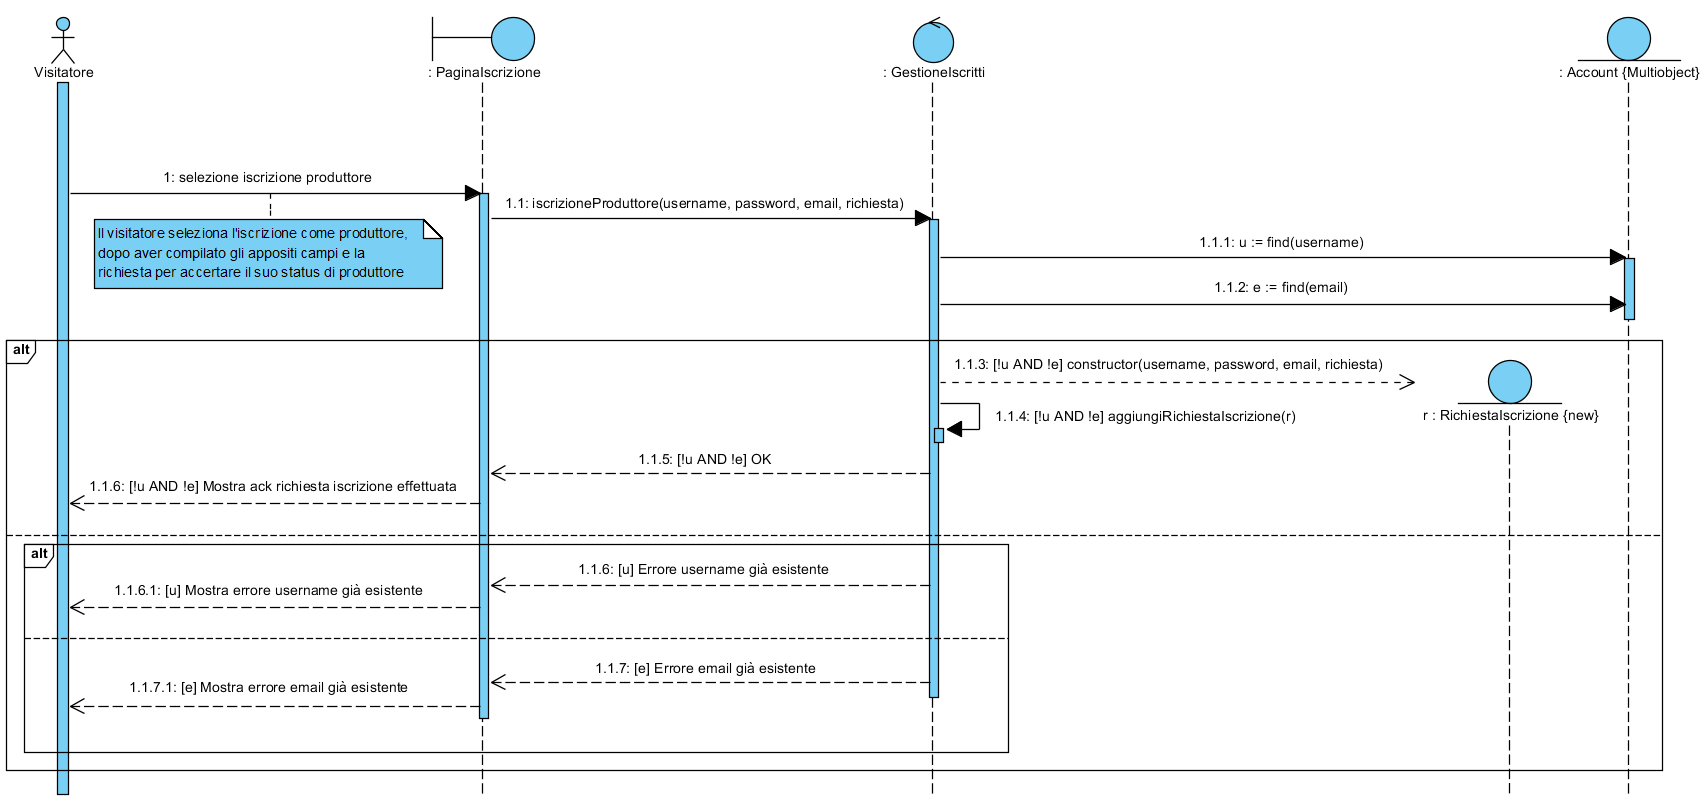
\includegraphics[width=\textwidth]{assets/visualParadigm/sequenza/iscrizioneProduttore}
\end{center}

\linkedSubsection{seq:iscrizioneUtente}
\begin{center}
			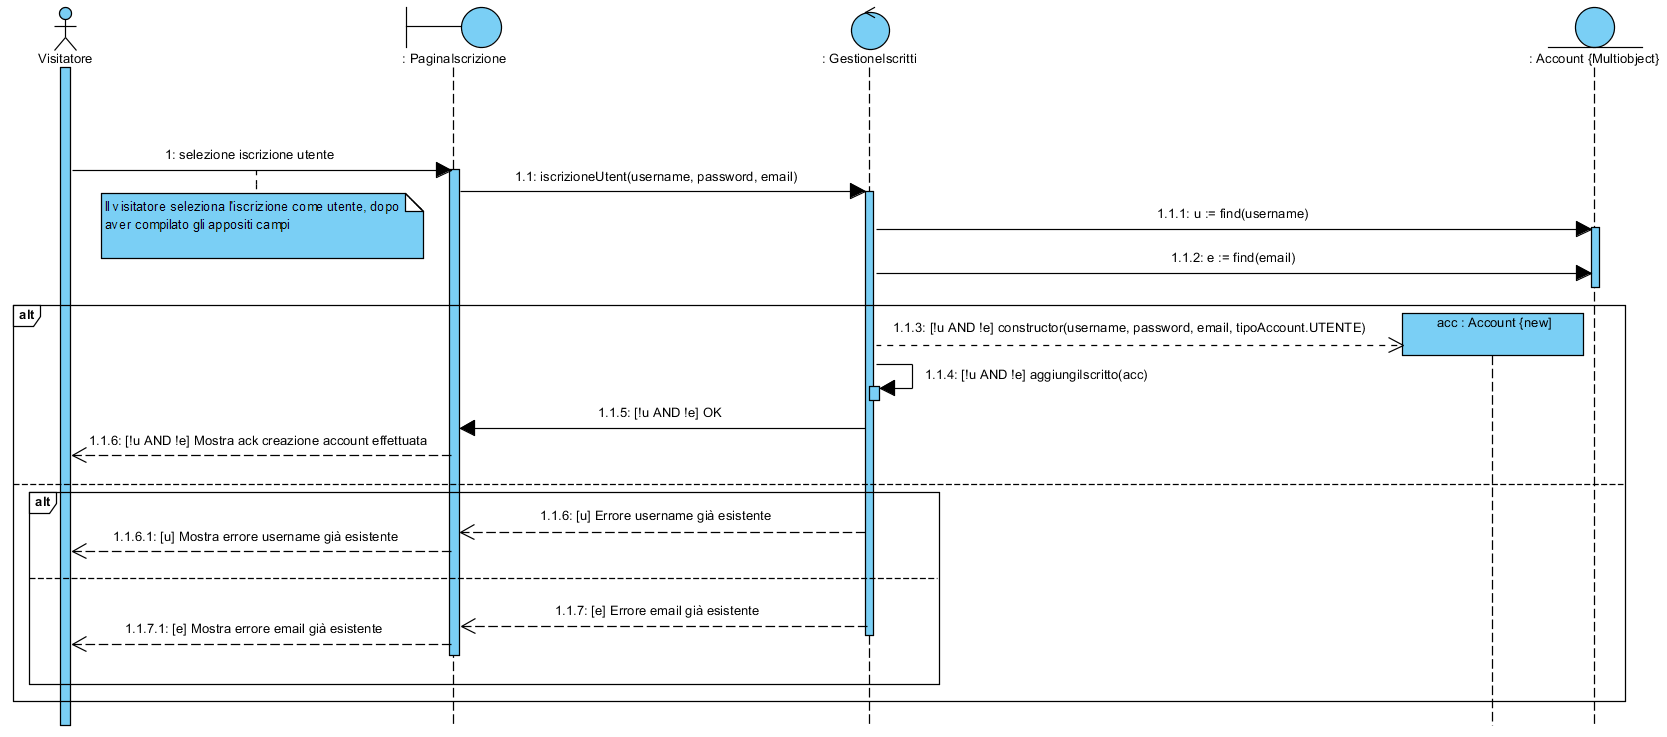
\includegraphics[width=\textwidth]{assets/visualParadigm/sequenza/iscrizioneUtente}
\end{center}

\linkedSubsection{seq:approvazioneIscrizione}
\begin{center}
			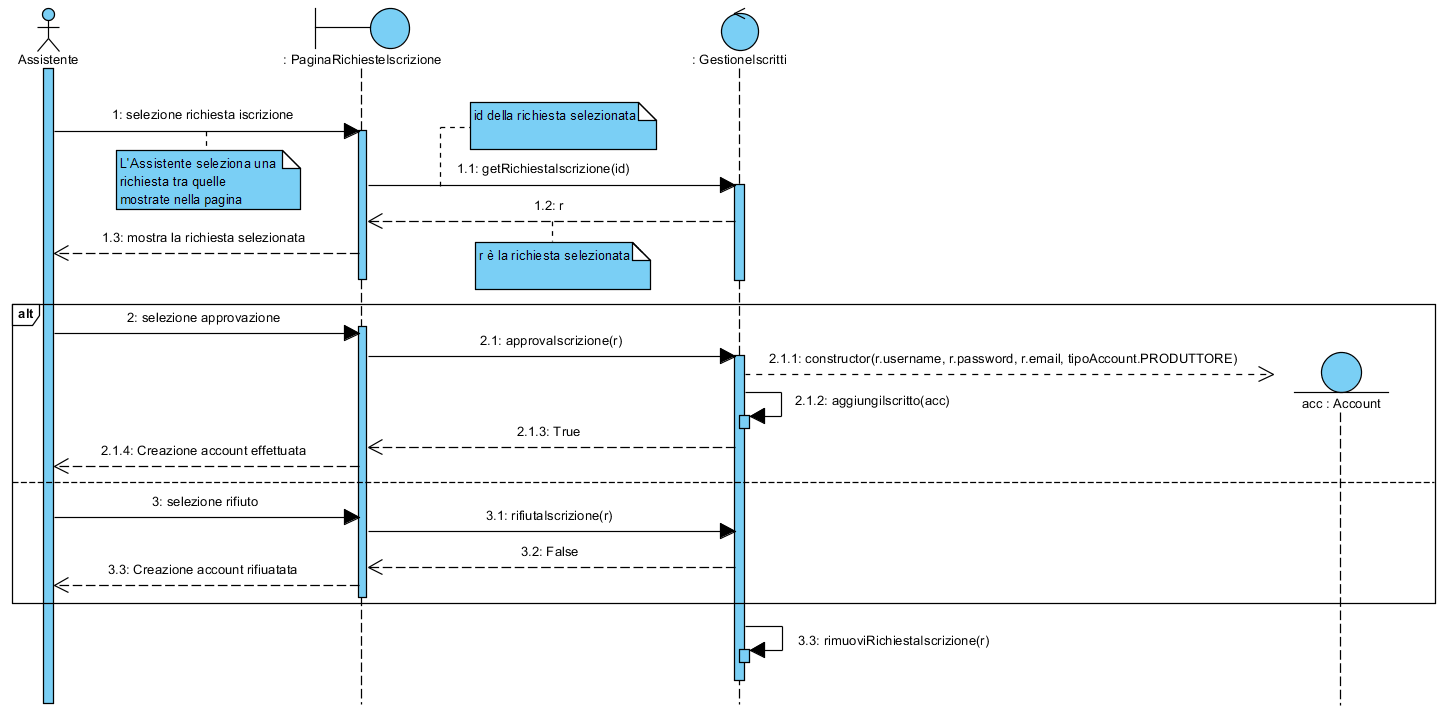
\includegraphics[width=\textwidth]{assets/visualParadigm/sequenza/approvazioneIscrizione}
\end{center}

\linkedSubsection{seq:inserimentoSchedaProdotto}
\begin{center}
			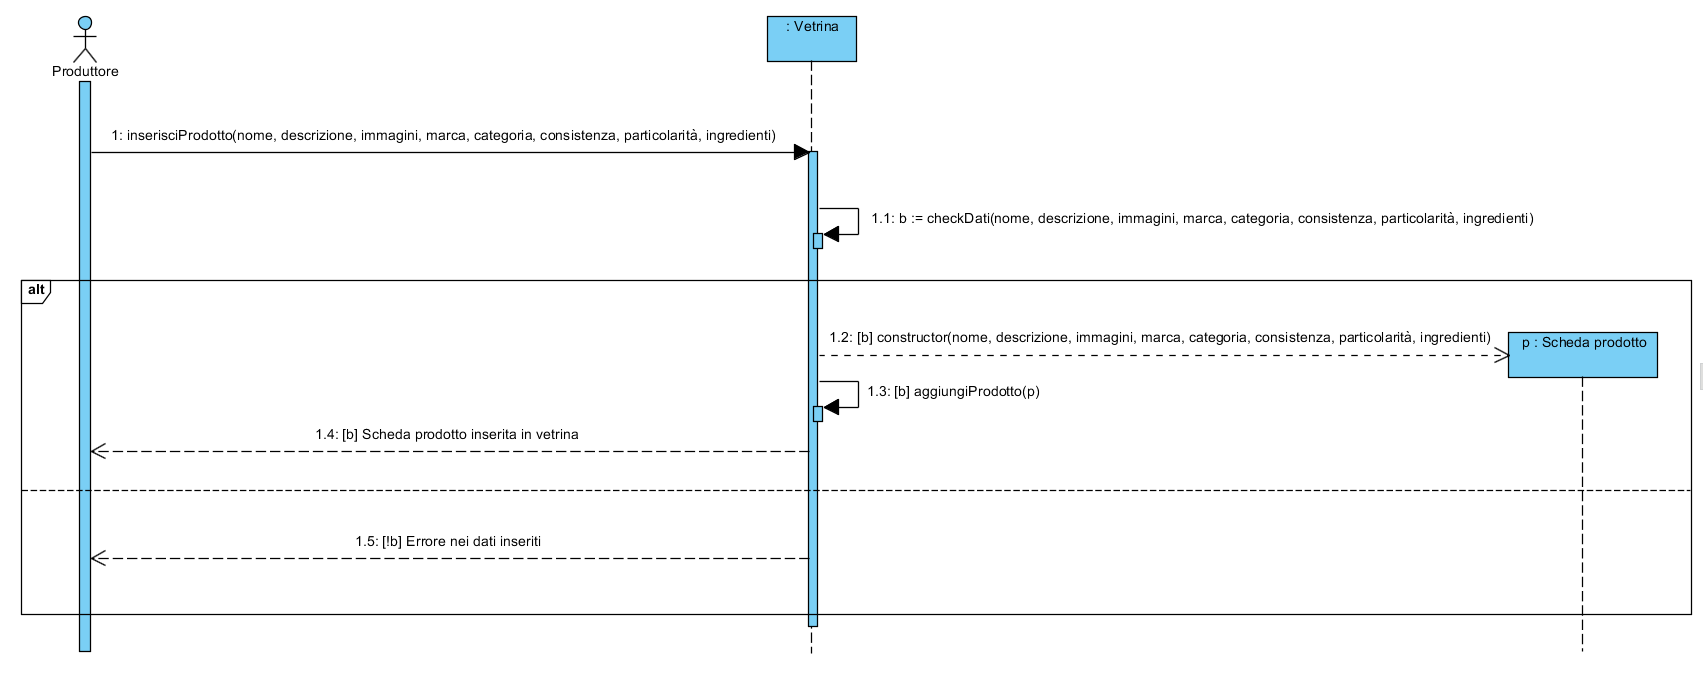
\includegraphics[width=\textwidth]{assets/visualParadigm/sequenza/inserimentoSchedaProdotto}
\end{center}

\linkedSubsection{seq:inserimentoValutazione}
\begin{center}
			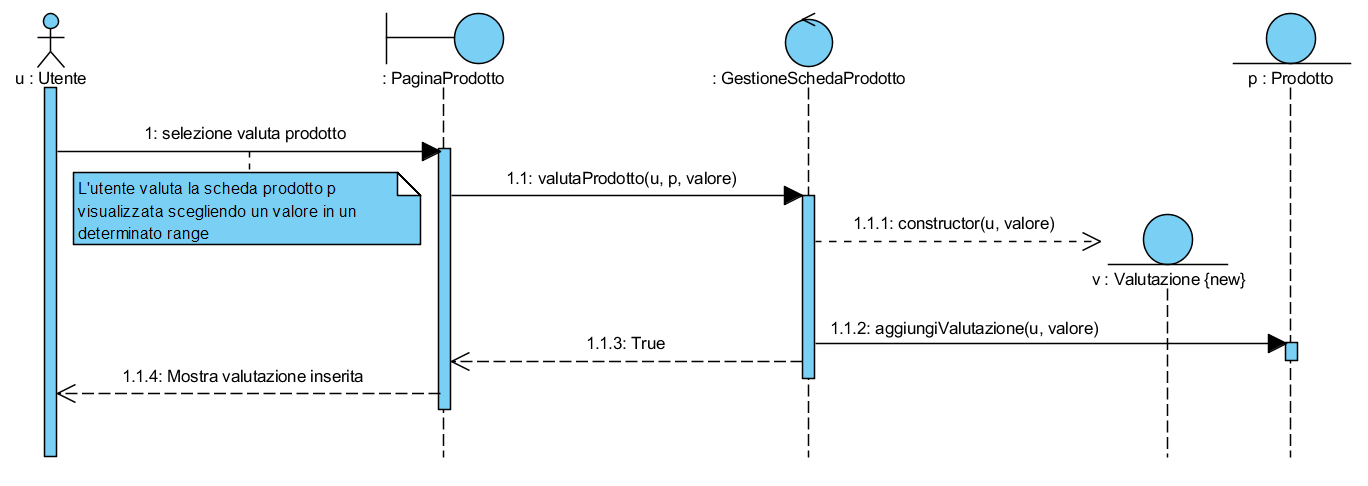
\includegraphics[width=\textwidth]{assets/visualParadigm/sequenza/inserimentoValutazione}
\end{center}

\linkedSubsection{seq:inserimentoRecensione}
\begin{center}
			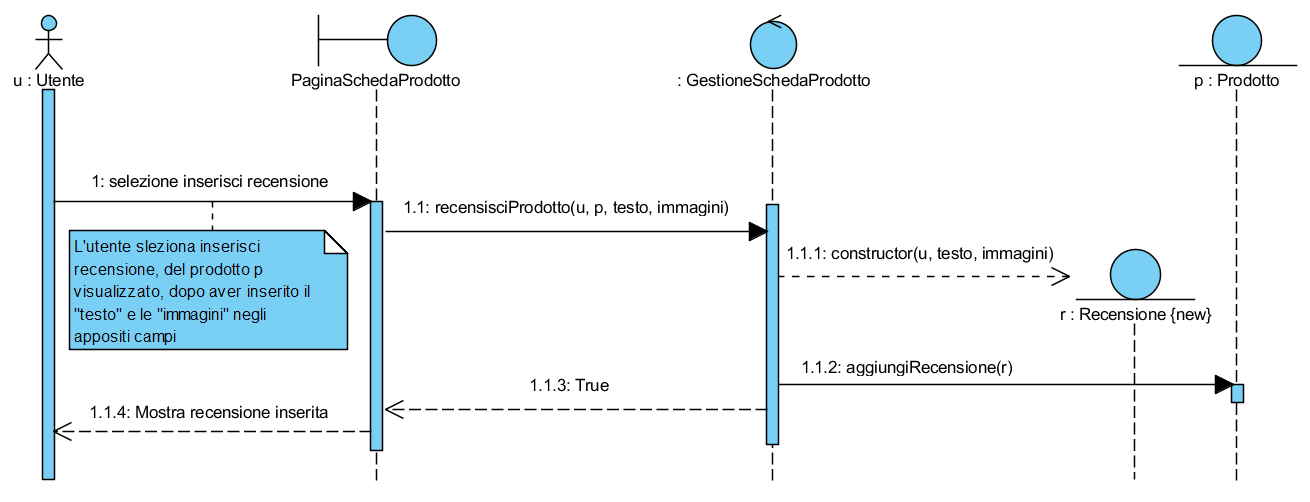
\includegraphics[width=\textwidth]{assets/visualParadigm/sequenza/inserimentoRecensione}
\end{center}

\linkedSubsection{seq:rimuoviRecensione}
\begin{center}
			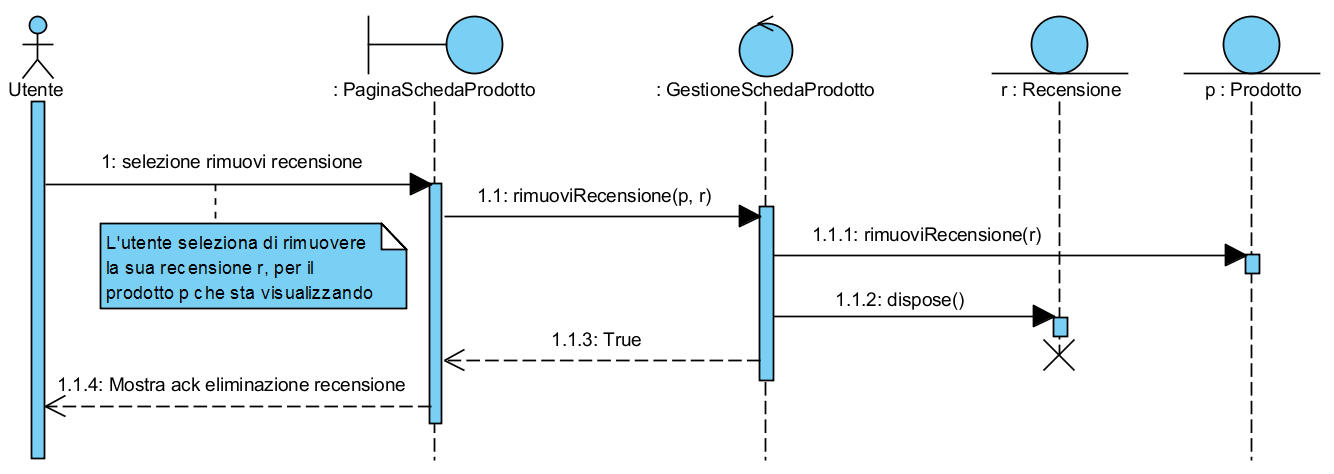
\includegraphics[width=\textwidth]{assets/visualParadigm/sequenza/rimuoviRecensione}
\end{center}

\linkedSubsection{seq:commentoRecensione}
\begin{center}
			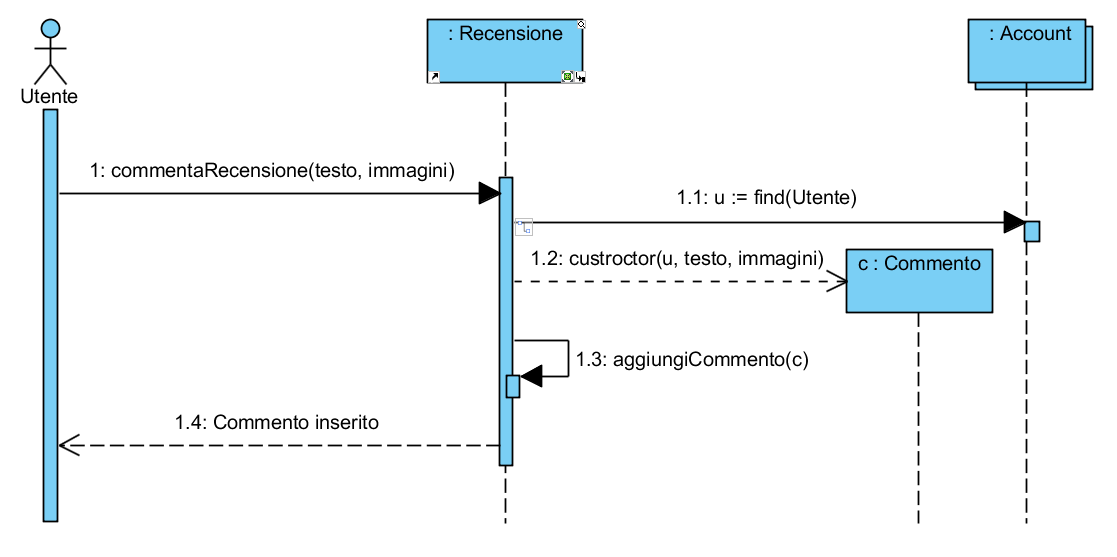
\includegraphics[width=\textwidth]{assets/visualParadigm/sequenza/commentoRecensione}
\end{center}

\linkedSubsection{seq:giudicaRecensione}
\begin{center}
			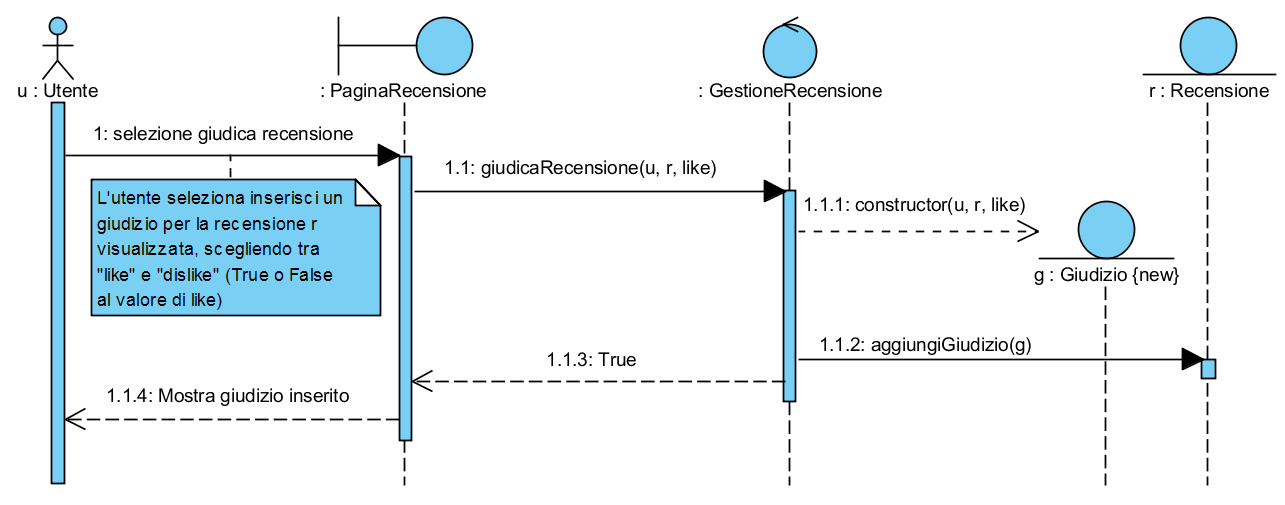
\includegraphics[width=\textwidth]{assets/visualParadigm/sequenza/giudicaRecensione}
\end{center}

\linkedSubsection{seq:ricerca}
\begin{center}
			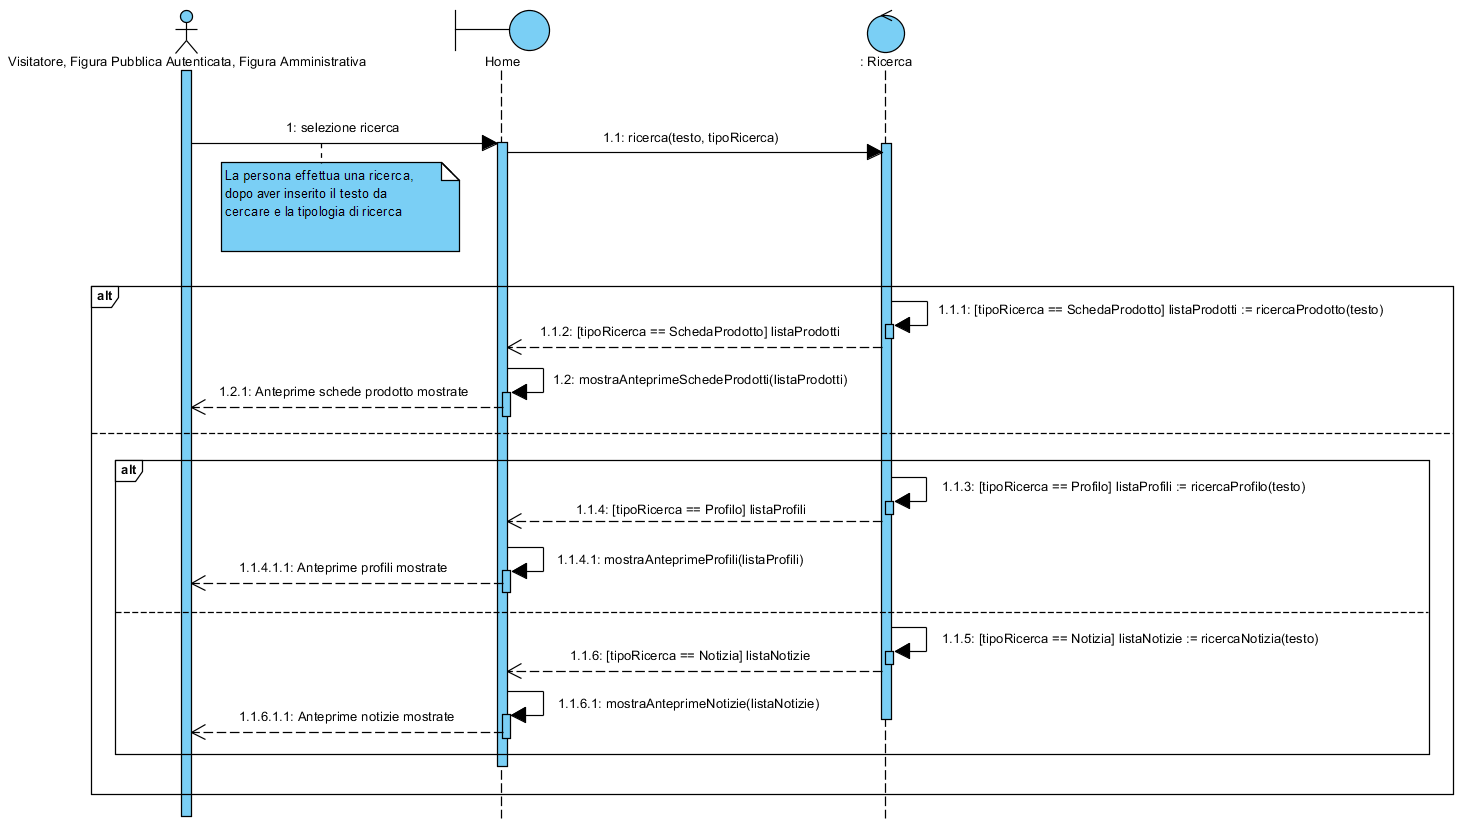
\includegraphics[width=\textwidth]{assets/visualParadigm/sequenza/ricerca}
\end{center}


\begin{comment}
-	CU.A.1 - Login
-	CU.A.3 - Logout
-	CU.B.1 - Iscrizione tramite modulo
-	CU.B.2 - Iscrizione tramite Social Network
-	CU.B.3 - Iscrizione tramite approvazione
-	CU.B.4 - Approvazione iscrizione
-	CU.C.5 - Inserimento scheda prodotto

	CU.G.1 - Inserimento valutazione
	CU.H.1 - Inserimento recensione
	CU.H.4 - Commento a recensione
	CU.H.5 - Giudizio recensione

-	CU.K.1 - Ricerca prodotto
-	CU.K.2 - Ricerca profilo
-	CU.K.3 - Ricerca notizia
-	CU.M.1 - Mostra vetrina
-	CU.M.2 - Mostra scheda prodotto
-	CU.M.4 - Mostra recensione
-	CU.M.5 - Mostra profilo pubblico
-	CU.M.6 - Mostra notizia
\end{comment}
